\chapter{Wykorzystanie urządzeń mobilnych i nawigacji satelitarnej do treningów biegowych}\label{chap:wykorzystanie_urzadzen_mobilnych}
\section{Nawigacja satelitarna}\label{section:nawigacja-satelitarna}
Nawigacja satelitarna jest systemem, który pozwala ustalić pozycję punktu w przestrzeni. Zasada jej działania opiera się na pomiarze odległości pomiędzy odbiornikiem reprezentującym punkt, którego pozycja ma zostać ustalona, a satelitami znajdującymi się na orbicie okołoziemskiej. Wyznaczając odległość pomiędzy tylko jedną satelitą a odbiornikiem, możliwe jest stwierdzenie, że poszukiwany punkt znajduje się gdzieś na powierzchni pewnej sfery o środku równym położeniu satelity w chwili wysłania sygnału oraz promieniowi równemu wyznaczonej odległości. Analogicznie, mając dostęp do dwóch satelitów, można otrzymać dwie sfery. Odbiornik znajduje się wtedy na okręgu powstałym z przecięcia obu sfer. Choć pozycja odbiornika jest uściślona względem pierwszego przypadku, to nadal nie można ustalić jej dokładnej pozycji. Skorzystanie z trzeciego satelity sprawia, że przecięcie wszystkich sfer wyznacza tylko dwa punkty, w których może znajdować się antena odbiornika. Jeden z tych punktów znajduje się bardzo wysoko nad ziemią, dlatego można go pominąć. W ten sposób możliwe jest ustalenie dokładnej pozycji odbiornika w dwóch wymiarach. Chcąc poznać także wysokość na której znajduje się punkt, konieczne jest skorzystanie z minimum czterech satelitów  \cite{gps2}. Pozycja użytkownika ustalona w dwóch wymiarach jest wystarczająca do przeprowadzenia procesu wirtualnej rywalizacji. Automatyczne przypisanie cechy reprezentującej poziom terenu, przez który przebiega trasa, wymaga jednak informacji o pozycji użytkownika w trzech wymiarach.

Do pewnego momentu wspieranie treningów za pomocą danych pochodzących z nawigacji satelitarnej wymagało zakupu przyrządu przeznaczonego konkretnie do tego celu. Intensywny rozwój technologiczny sprawił jednak, że moduł nawigacji satelitarnej zaczął być powszechnie stosowany w telefonach komórkowych, a więc jego posiadanie stało się niezwykle powszechne. Warto zaznaczyć, że Globalny System Pozycyjny (GPS) jest niekiedy błędnie uogólniany do pojęcia nawigacji satelitarnej, gdy tak naprawdę jest on jedynie jednym z kilku istniejących systemów:
\begin{itemize}
\item{GPS} - amerykański system nawigacji, który jako pierwszy został oddany do użytku. W chwili obecnej w jego skład wchodzi 30 satelitów, które mogą osiągnąć dokładność rzędu 5 metrów. Zdobył ogromną popularność i można stwierdzić, że jest on jednym z największych osiągnięć technicznych ubiegłego wieku \cite{gpsgov},
\item{GLONASS} - system nawigacji stworzony przez Rosję. Składa się z 24 satelitów, które zastosowaniom cywilnym pozwalają na osiągnięcie dokładności około pięciu metrów \cite{gps2},
\item{BeiDou} - chiński system nawigacyjny. Docelowo w jego obrębie ma działać 35 satelitów pozwalających osiągnąć dokładność około dziesięciu metrów \cite{gps2,baidu1},
\item{Galileo} - europejski system nawigacji, który nadal jest w fazie budowy. Zakłada się, że jego precyzja będzie wynosić 4 metry. Zakończenie prac planowane jest na rok 2020 \cite{stronkagps1,gps2}.
\end{itemize}
Precyzja systemów nawigacji używanych obecnie w urządzeniach mobilnych sięga kilka metrów. Czynniki takie jak niekorzystne warunki atmosferyczne mogą jednak mieć negatywny wpływ na dokładność \cite{gps2}, co należy mieć na uwadze podczas projektowania aplikacji przeznaczonej treningom biegowym.

\section{Działania na danych pochodzących z nawigacji satelitarnej}
\subsection{Obliczanie odległości pomiędzy dwoma punktami geograficznymi}\label{chap:haversine}
Do obliczenia odległości pomiędzy dwoma punktami na sferze można skorzystać z \textbf{formuły haversine} \cite{haversine}. Jej wzór prezentuje się następująco:\\
\begin{equation}\label{eq:haversine11}
a = \sin ^2(\frac{\Delta  \phi}{2}) + cos  \phi_1 \cdot cos\phi_2 \cdot sin^2(\frac{\Delta \lambda}{2})
\end{equation}
\begin{equation}\label{eq:haversine2}
c = 2 \cdot atan2( \sqrt{a}, \sqrt{1-a})
\end{equation}
\begin{equation}\label{eq:haversine3}
d = R \cdot c
\end{equation}
gdzie \(\phi\) jest szerokością geograficzną, \(\lambda\) długością geograficzną, \(R\) średnim promieniem Ziemi wynoszącym w zaokrągleniu 6371 kilometrów. Wzór zakłada, że miary wszystkich kątów podane są w radianach.

\subsection{Wyznaczanie punktu oddalonego o podany dystans i kąt od punktu początkowego}
Znając punkt początkowy, kierunek oraz odległość możliwe jest wyznaczenie punktu końcowego za pomocą następującego wzoru \cite{haversine}:
\begin{equation}\label{eq:haversine_generowanie_punktu}
\begin{cases}\varphi_2=asin(sin{ \varphi_1 } \cdot cos{ \delta } + cos{\varphi_1} \cdot sin{\delta} \cdot cos{ \theta })\\
\lambda_2 = \lambda_1 + atan2(sin \theta \cdot sin \delta \cdot cos \varphi_1, cos \delta -sin \varphi_1 \cdot sin  \varphi_2 )
\end{cases}
\end{equation}
gdzie \(\phi\) jest szerokością geograficzną, \(\lambda\) długością geograficzną, \(\theta\) określonym względem północy, zgodnie ze wskazówkami zegara kierunkiem wyrażonym w radianach, \(d\) odległością od punktu początkowego,
\(R\) średnim promieniem Ziemi wynoszącym w zaokrągleniu 6371 kilometrów, \(\delta\) odległością kątową (\(\frac{d}{R}\)). Wzór zakłada, że miary wszystkich kątów podane są w radianach.

\section{Możliwe problemy i sposoby ich rozwiązania}
Wykorzystywanie danych pochodzących z nawigacji satelitarnej do celu, w którym precyzja jest niezwykle istotna może przysporzyć pewnych problemów. W tym rozdziale opisano możliwe do napotkania problemy oraz propozycje ich rozwiązania.
\subsection{Automatyczne określenie poziomu terenu w przypadku dostępu do jedynie trzech satelitów}\label{chap:problem-poziom-terenu}
Jak wspomniano w podrozdziale \ref{section:nawigacja-satelitarna}, mając jednoczesny dostęp do trzech satelitów, pomimo znajomości pozycji użytkownika na mapie, nie jest możliwe określenie jego wysokości nad poziomem morza. Z tego powodu nie można dokonać automatycznego określenia cechy trasy, która daje biegaczowi informacje na temat tego, czy możliwe jest napotkanie na niej jakichś podbiegów lub zbiegów. Brakująca wysokość może zostać ustalona przy pomocy zewnętrznych serwisów udostępniających brakującą daną na podstawie szerokości oraz długości geograficznej. Przykładem narzędzia udostępniającego tę funkcjonalność jest serwis Google Maps \cite{googlemaps}. Biorąc pod uwagę, że urządzenia mobilne są obecnie w stanie obsługiwać różne systemy nawigacji satelitarnej, dla których ilość dostępnych satelitów przekracza 20, prawdopodobieństwo posiadania jednoczesnego kontaktu z mniej niż czterema satelitami, a tym samym niemożności określenia wysokości użytkownika nad poziomem morza jest stosunkowo niskie. Z tego względu w aplikacji tworzonej w ramach niniejszej pracy nie zaimplementowano pobierania wysokości z zewnętrznego serwisu. W przypadku gdy ilość jednocześnie dostępnych satelitów nie przekracza trzech, omawiana cecha trasy jest ustalana przez użytkownika.
\subsection{Wahania pozycji przy braku ruchu}\label{chap:wahania-pozycji}
Pozycja wyznaczana przy użyciu nawigacji satelitarnej obarczona jest kilkumetrowym błędem. Oznacza to, że dokonując kilku odczytów, lokalizacja okaże się za każdym razem inna, pomimo faktu że w rzeczywistości odbiornik znajduje się za każdym razem w tym samym miejscu. Przykładowe odczyty dla nieporuszającego się odbiornika zostały przedstawione w tabeli \ref{table:punktygps}, a ich wizualizację na mapie umieszczono na rysunku \ref{fig:mapka_punktygps}. Odległość pomiędzy skrajnie oddalonymi od siebie punktami wynosi niespełna 10 metrów. Rozwiązaniem tego problemu jest branie pobranego punktu pod uwagę tylko wtedy, gdy jego odległość od punktu go poprzedzającego przekracza pewną wartość. Użytkownik nieporuszający się nie spełni tego warunku, co zapobiegnie wystąpieniu przedstawionego problemu.

\begin{table}[h!]
\parbox{\dimexpr\linewidth-8cm\relax}{\centering%
\captionsetup{justification=centering}
\captionof{table}{Współrzędne nieporuszającego się odbiornika.}\label{table:punktygps}
\begin{tabular}{|c|c|c|}
\hline
%\textbf{L.p.} & \textbf{Szerokość \newline geograficzna} & \textbf{Długość geograficzna} \\
L.p. & \begin{tabular}[c]{@{}c@{}}Szerokość\\geograficzna\end{tabular} & \begin{tabular}[c]{@{}c@{}}Długość\\geograficzna\end{tabular} \\
\hline
1. & 51.95 & 19.204412\\\hline
2. & 51.949984 & 19.204416\\\hline
3. & 51.949975 & 19.204412\\\hline
4. & 51.949966 & 19.204412\\\hline
5. & 51.949942 & 19.204414\\\hline
6. & 51.949922 & 19.204446\\\hline
7. & 51.949921 & 19.204449\\\hline
8. & 51.949918 & 19.204456\\\hline
\end{tabular}
\label{tab:xt}}
\parbox{6cm}{%
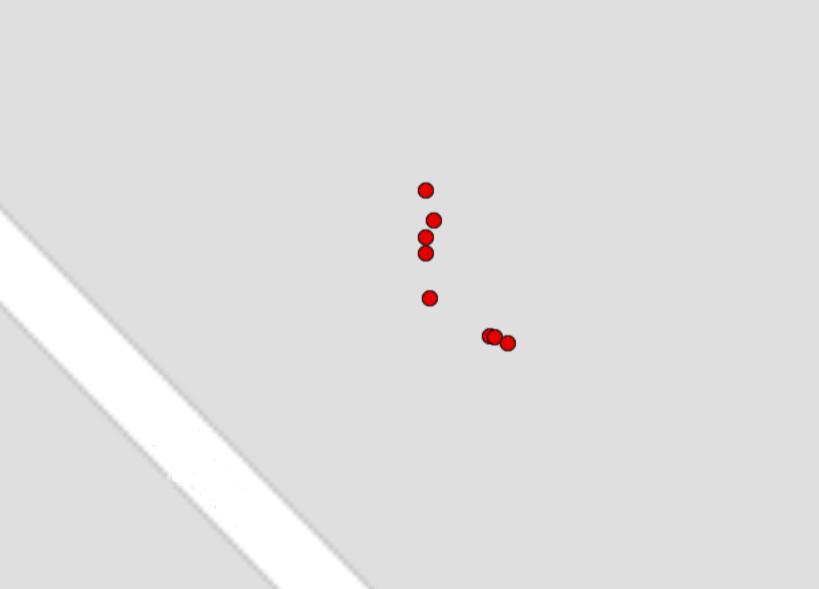
\includegraphics[width=3in]{img/mapka_punktygps.png}
\captionsetup{justification=centering}
\captionof{figure}{Wizualizacja współrzędnych nieporuszającego się odbiornika na mapie. [Opracowanie własne]}
\label{fig:mapka_punktygps}
}
\end{table}%

Zignorowanie powyższego zjawiska, mogłoby doprowadzić do bardzo niekorzystnej sytuacji. Gdyby osoba tworząca trasę zatrzymała się w trakcie treningu, na przykład w celu odpoczynku lub zawiązania buta, zapisany przebieg treningu zawierałby skupisko fałszywych punktów. W celu wyeliminowania tego zagrożenia, podczas tworzenia trasy brane są pod uwagę tylko te punkty, które są oddalone od poprzedniego o więcej niż 15 metrów. Dzięki temu chwilowe zatrzymanie się podczas treningu, nie powoduje powstania przekłamań w generowanej trasie.
\subsection{Zapobieganie oszustwom}
Opieranie rywalizacji biegowej jednie na danych pobieranych z systemów nawigacji satelitarnej, sprawia że jej uczciwość może być zaburzona w stosunkowo łatwy sposób. Nic nie stoi na przeszkodzie, aby do pokonania trasy użyć chociażby roweru. Możliwe jest także manualne wprowadzanie danych lokalizacyjnych do urządzenia \cite{fakegps}, co pozwoli uzyskać dowolnie dobry wynik bez podejmowania jakiejkolwiek aktywności fizycznej. Zagrożenia tego można uniknąć na dwa sposoby:
\begin{itemize}
\item{\textbf{Porównywanie osiąganych przez użytkowników rezultatów z wynikami najlepszych na świecie biegaczy}} - Zapisanie w aplikacji zbioru światowych rekordów biegowych na konkretnych dystansach i porównywanie ich do wyników uzyskiwanych przez użytkowników jest pierwszym ze sposobów na zapobieganie oszustwom. Rezultaty znacząco lepsze od tych, które zostały osiągnięte na atestowanych zawodach z całą pewnością mogą zostać uznane jako osiągnięte nieuczciwie. Choć rozwiązanie to zapobiegnie zapisywaniu w rankingu czasów trasy, które są wręcz niemożliwe do osiągnięcia, nie sprawdzi się w przypadkach gdy sfałszowany wynik mieści się w granicach zdrowego rozsądku.
\item{\textbf{Skorzystanie z czujników dostępnych w urządzeniu}} - Akcelerometr oraz żyroskop są jednymi z wielu czujników umieszczanych w produkowanych obecnie telefonach komórkowych. Ich zadaniem jest mierzenie przyspieszenia liniowego oraz położenia kątowego \cite{czujniki}. Umożliwiają zatem pozyskanie informacji o ruchach jakim poddane jest urządzenie w trakcie trwania treningu. Opracowanie odpowiedniego algorytmu oraz skorzystanie z sieci neuronowych pozwoliłyby stwierdzić, czy dane pobrane z czujników w czasie odbywania treningu, zgadzają się z tymi, które generowane są w czasie biegu i na tej podstawie dokonać akceptacji lub unieważnienia próby użytkownika. W przeciwieństwie do poprzedniego podejścia, bieżące rozwiązanie okazałoby się skuteczne także w przypadkach, w których dane lokalizacyjne zostały wprowadzone do urządzenia manualnie oraz gdy osiągnięty na trasie rezultat nie jest lepszy niż ogólnoświatowe rekordy. Rozwiązanie tego problemu obejmuje zagadnienia z dziedziny sztucznej inteligencji i wykracza poza zakres niniejszej pracy, dlatego też nie zostało zaimplementowane w tworzonej aplikacji.
\end{itemize}

\section{Istniejące rozwiązania w dziedzinie aplikacji treningowych}\label{chap:istniejace}
Na rynku aplikacji znajduje się wiele aplikacji, których przeznaczeniem jest wspieranie treningów biegowych. Pozwalają one użytkownikom na dogłębną analizę aktywności sportowych oraz śledzenie treningów zarówno swoich jak i udostępnianych przez innych biegaczy. Funkcjonalności te są bardzo powszechne. Nie udało się znaleźć aplikacji treningowej, która w pełni oferuje funkcjonalność zawartą w rozwiązaniu, które budowane jest w ramach niniejszej pracy, dlatego do niniejszego przeglądu wybrano trzy przykłady aplikacji, których zakres działania jest jak najbardziej do niej zbliżony, a jednocześnie cieszących się wysoką oceną oraz popularnością w sklepie z aplikacjami Google Play \cite{googleplay}. 
\subsection{Endomondo}
Jedną z najwcześniej wydanych (pierwsze wersja została udostępniona w listopadzie 2007 roku), a zarówno najbardziej popularnych na świecie aplikacji jest Endomondo \cite{endomondo}.  Pozwala na śledzenie aktywności w ponad 60 dyscyplinach sportowych, włączając w to bieganie. W aplikacji rozwinięto aspekt społecznościowy - znajomi mają możliwość wzajemnego przeglądania historii swoich treningów. Ich statystyki mogą być także udostępniane na mediach społecznościowych. Ponadto istnieje możliwość tworzenia własnych tras, które inni biegacze mogą następnie przeglądać w formie listy i używać do własnych treningów. Niestety możliwe jest zobaczenie tylko całego zbioru tras, znajdujących się w pewnej nieznanej odległości od użytkownika. Stanowi to problem, ponieważ nie mogąc określić dokładnie obszaru wyszukiwania, biegacze nie są pewni, czy zobaczyli już wszystkie trasy, które mogłyby ich potencjalnie zainteresować czy może istnieje ich więcej, ale znajdują się poza nieznanym obszarem wyszukiwania. Producent nie udostępnił także możliwości filtrowania wyników wyszukiwania ze względu na długość trasy, twardość nawierzchni czy poziom terenu. Podczas tworzenia trasy zapisywana jest co prawda jej całkowita długość, jednak służy ona tylko poinformowaniu użytkownika, a nie wyszukiwaniu. Aplikacja nie pozwala także na jakiekolwiek porównywanie wyników, które biegacze osiągają na trasie.
\subsection{Strava}
Strava \cite{strava} jest aplikacją, która w momencie pisania niniejszej pracy wspiera treningi w 24 dyscyplinach sportowych. Oprócz podstawowej funkcjonalności aplikacji treningowych, oferuje także analizę treningów na podstawie rozmaitych statystyk i wykresów. Aplikacja umożliwia także funkcję tworzenia i zapisywania tras. Oprócz samego jej przebiegu, zapisywana jest także jej długość oraz poziom terenu. Niestety, tak jak w przypadku aplikacji Endomondo, producent nie umożliwił filtrowania tras według żadnej z tych cech. Podczas przeglądania tras, ukazują się one na interaktywnej mapie, którą można przesuwać. Nie występuje tutaj zatem znany z Endomondo problem niemożności określenia obszaru, w którym wyszukiwane są trasy. Rozszerzenie obszaru poszukiwania ogranicza się do przesunięcia mapy na ekranie urządzenia. Zapisywanie czasów użytkowników którzy ukończyli trasę na serwerze, pozwala użytkownikom na wyświetlenie rankingu trasy i porównanie swojej dyspozycji do innych biegaczy. Funkcjonalność ta daje poczucie pewnego rodzaju rywalizacji, jednak sprawdzenie uzyskanego wyniku możliwe jest dopiero po ukończeniu treningu, użytkownik nie otrzymuje na ten temat informacji w czasie jego trwania.
\subsection{MapMyRun}
Przeznaczeniem aplikacji MapMyRun \cite{mapmyrun} jest przede wszystkim śledzenie aktywności związanych ze spacerowaniem i bieganiem. W tym przykładzie użytkownicy także mają możliwość przeglądania i analizowania swoich poprzednich treningów. Usprawnieniem jest fakt, iż trasy można filtrować na podstawie ich długości. Zabrakło niestety filtra poziomu terenu, mimo że informacja ta jest zapisywana podczas tworzenia trasy. Podczas wyszukiwania tras pojawia się problem znany z aplikacji Endomondo - prezentowane trasy należą do obszaru, którego granice oddalone są od użytkownika o nieznaną odległość, przez co biegacze nie są pewni czy zostały im wyświetlone wszystkie godne uwagi trasy czy może część z nich znajduje się poza obszarem poszukiwań. Element rywalizacji jest zorganizowany podobnie jak w aplikacji Strava - wyniki osiągane przez użytkowników są zapisywane na serwerze, dzięki czemu mają oni możliwość sprawdzenia swojej dyspozycji po zakończonym treningu.